%!TEX root = ../talk.tex

\section{MXNet}\label{sec:MxNet}

%%%

\frameinlbffalse

{
\usebackgroundtemplate{
\tikz[overlay,remember picture] \node[opacity=0.8, xshift=-3.5cm, at=(current page.east)] {

\includegraphics[width=0.35\paperwidth]{figures/mxnet_logo.jpg}
};}

\begin{frame}[plain]
\frametitle{\S\ref{sec:MxNet}. \insertsection}
\listofframes
\end{frame}
\addtocounter{framenumber}{-1} % this page does not count

}

\frameinlbftrue

%%%
\subsection{Programming interface}
%%%

\begin{frame}
  \MyLogo
  \frametitle{General Comments}  

\begin{enumerate}
%
\item Used to power Amazon Web Services (AWS)
%
\item Support many different applications (e.g. computer vision, natural language processing,  speech recognition, unsupervised machine learning, support embedded APIs, visualization)
%
\item Mixed programming style: imperative and declarative
\begin{itemize}
\item Light-weighted (around 50K lines of core code)
\item Data parallelism with multi-devices: 88\% scalability with 256 GPUs
\item Support many front-ends, including JavaScript (run on web browsers)
\item Provide intermediate-level and high-level interface modules
\item Provide abundant IO functions 
%
\end{itemize}
%
\item Fully compatible with Torch: modules and operators
%
\item Visualize neural network graphs
\begin{itemize}
\item Call mx.viz.plot\_network( )
\end{itemize}
%
\item Not well documented, code not easy to read
%
\end{enumerate}

\end{frame}

%%%
\subsection{Simple examples}
%%%

\begin{frame}[fragile]
  \MyLogo
  \frametitle{Example: SoftMax in MXNet}  

\begin{lstlisting}[language=python]
import os, gzip, struct
import numpy as np
import mxnet as mx

# Read data from the MNIST dataset
def read_data(label_url, image_url):
    with gzip.open(label_url) as flbl:
        magic, num = struct.unpack(">II", flbl.read(8))
        label = np.fromstring(flbl.read(), dtype=np.int8)
    with gzip.open(image_url, 'rb') as fimg:
        magic, num, row, col = struct.unpack(">IIII", fimg.read(16))
        image = np.fromstring(fimg.read(),dtype=np.uint8).reshape(len(label),row,col)
    return (label, image)

train_lbl_file = 'train-labels-idx1-ubyte.gz'
train_img_file = 'train-images-idx3-ubyte.gz'
train_lbl, train_img = read_data(train_lbl_file, train_img_file)

test_lbl_file = 't10k-labels-idx1-ubyte.gz'
test_img_file = 't10k-images-idx3-ubyte.gz'
test_lbl,  test_img  = read_data(test_lbl_file, test_img_file)

# Create data iterators for MXNet
def to4d(img):
    return img.reshape(img.shape[0], 1, 28, 28).astype(np.float32)/255

batch_size = 100
train_iter = mx.io.NDArrayIter(to4d(train_img), train_lbl, batch_size, shuffle=True)
test_iter  = mx.io.NDArrayIter(to4d(test_img), test_lbl, batch_size)

\end{lstlisting}

\end{frame}

%%%

\begin{frame}[fragile]
  \MyLogo
  \frametitle{Example: SoftMax in MXNet (Cont)}  

\ContinueLineNumber
\scriptsize{
\begin{lstlisting}[language=python]
# Define the network
data = mx.sym.Variable('data') # Create a place holder variable for the input data
data = mx.sym.Flatten(data=data)# Flatten the data from 4-D shape into 2-D
fc1  = mx.sym.FullyConnected(data=data, name='fc1', num_hidden=64) 
act1 = mx.sym.Activation(data=fc1, name='relu1', act_type="relu")
fc2  = mx.sym.FullyConnected(data=act1, name='fc2', num_hidden = 32)
act2 = mx.sym.Activation(data=fc2, name='relu2', act_type="relu")
fc3  = mx.sym.FullyConnected(data=act2, name='fc3', num_hidden=10)
out  = mx.sym.SoftmaxOutput(data=fc3, name='softmax')
mod  = mx.mod.Module(out)

# Plot the network graph
mx.viz.plot_network(symbol=out, shape={'data': (batch_size, 1, 28, 28)}).view()

# Prepare output log infomation
import logging
logging.getLogger().setLevel(logging.INFO)

# Train the network
mod.fit(train_data=train_iter, eval_data=test_iter, num_epoch=25)

\end{lstlisting}
}

\vskip 50pt

\begin{center}
{\color{red}\scriptsize
https://github.com/dmlc/mxnet/blob/master/example/svm\_mnist/svm\_mnist.py
}
\end{center}

\end{frame}


%%%
\subsection{Visualization}
%%%

\begin{frame}
	\MyLogo
	\frametitle{Visualization of the SoftMax Example}  

\vskip -5pt
\begin{figure}[htbp] 
	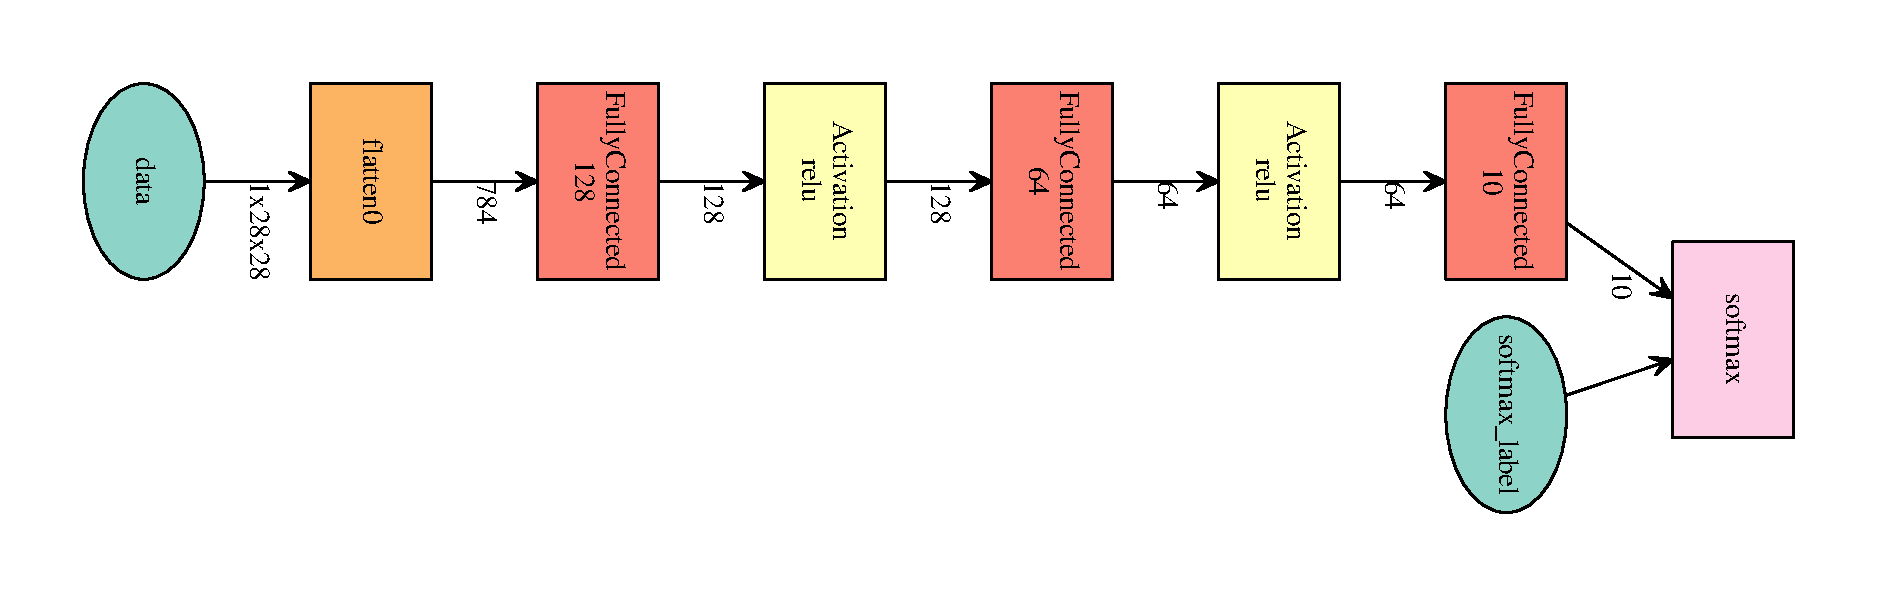
\includegraphics[height=0.65\linewidth]{figures/mxnet_graph.pdf} 
\end{figure}
	
\end{frame}